%% Introducción



\documentclass[serif, aspectratio=169]{beamer}
\usepackage{bookmark}
%\documentclass[serif]{beamer}  % for 4:3 ratio
\usepackage[T1]{fontenc} 
\usepackage{fourier}
\usepackage{hyperref}
\usepackage{bookmark}
\usepackage{latexsym,amsmath,xcolor,multicol,booktabs,calligra}
\usepackage{graphicx,listings,stackengine}
\usepackage[spanish]{babel}
%\setbeameroption{show notes on second screen=right} % Para la versión final desactivo esto.

\author{Alberto Daniel Lange}
\vspace{-3mm}
\title{Sistema de comunicaciones seguras \\ con segmentación virtual de dominios}
\subtitle{\small Avance de proyecto}
\institute{
    Dirección: Juan Ignacio Vaccarezza \\
    Codirección: Santiago Pérez Ghiglia \\
    \vspace{2mm}
    Ingeniería en Telecomunicaciones \\
    Instituto Balseiro
}
\vspace{-7mm}
\date{\small 26 de febrero de 2025}
\usepackage{UoWstyle}

% defs
\def\cmd#1{\texttt{\color{red}\footnotesize $\backslash$#1}}
\def\env#1{\texttt{\color{blue}\footnotesize #1}}
\definecolor{deepblue}{rgb}{0,0,0.5}
\definecolor{deepred}{RGB}{153,0,0}
\definecolor{deepgreen}{rgb}{0,0.5,0}
\definecolor{halfgray}{gray}{0.55}

\lstset{
    basicstyle=\ttfamily\small,
    keywordstyle=\bfseries\color{deepblue},
    emphstyle=\ttfamily\color{deepred},   
    stringstyle=\color{deepgreen},
    numbers=left,
    numberstyle=\small\color{halfgray},
    rulesepcolor=\color{red!20!green!20!blue!20},
    frame=shadowbox,
}


\begin{document}

% INICIO
\begin{frame} % LOGOS INSTITUCIONALES
    \titlepage
    \vspace*{-0.8cm}
\begin{columns}
    \begin{column}{0.25\textwidth}
        \begin{figure}
            \centering
            
\includegraphics[width=0.3\textwidth]{images/institucionales_cnea.png}
        \end{figure}
    \end{column}
    \begin{column}{0.25\textwidth}
        \begin{figure}
            \centering
            
\includegraphics[width=0.3\textwidth]{images/institucionales_IB.png}
        \end{figure}
    \end{column}
    \begin{column}{0.25\textwidth}
        \begin{figure}
            \centering
            
\includegraphics[width=0.5\textwidth]{images/institucionales_INVAP.png}
        \end{figure}
    \end{column}
    \begin{column}{0.25\textwidth}
        \begin{figure}
            \centering
            
\includegraphics[width=0.3\textwidth]{images/institucionales_cuyo.png}
        \end{figure}
        
    \end{column}
\end{columns}
\end{frame}


\begin{frame}    
\tableofcontents[sectionstyle=show,
subsectionstyle=show/shaded/hide,
subsubsectionstyle=show/shaded/hide]
\end{frame}

\section{Introducción}

\begin{frame}{Contexto}
            \begin{figure}
                \centering
                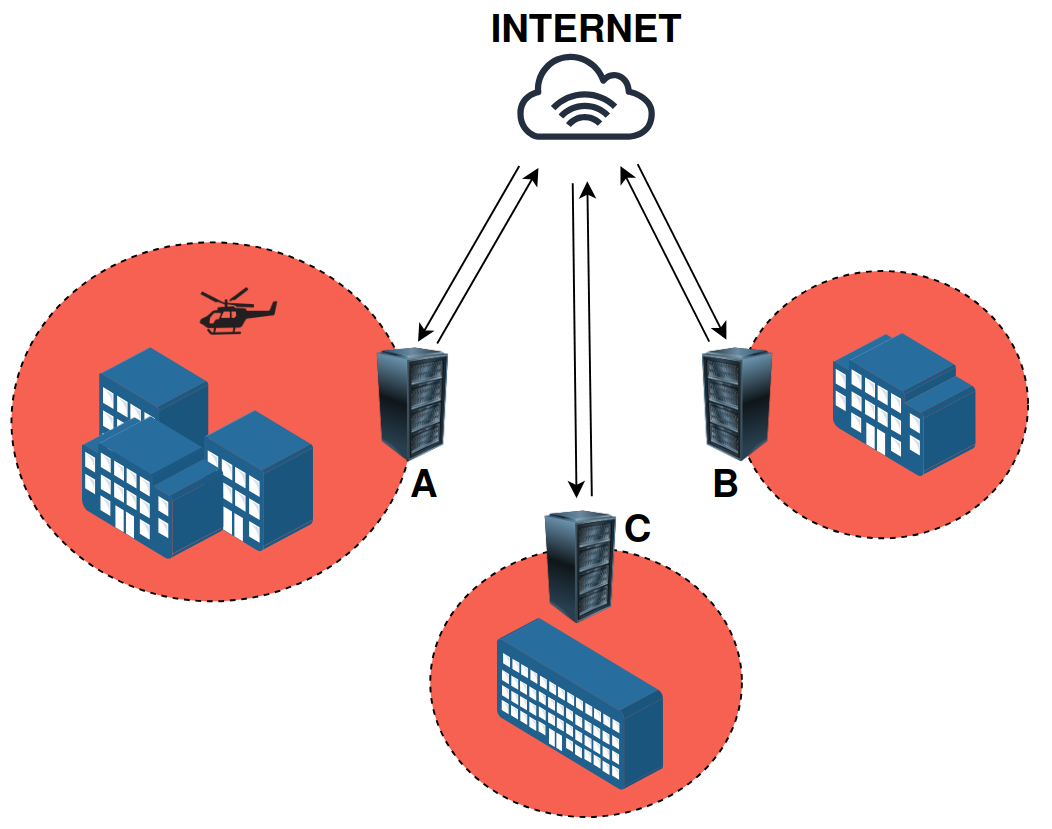
\includegraphics[width=0.5\textwidth]{images/conops.png}
                \caption{\centering Esquema simplificado de operación del sistema.}
            \end{figure}

    \note{Antes que nada quiero dar un pantallazo general de lo que se trata este proyecto. ¿A que nos referimos con sistema de comunicaciones seguras? Se trata del desarrollo de un dispositivo encriptador destinado a asegurar las comunicaciones entre sitios, es decir, que permita establecer una red privada virtual o VPN entre estos sitios.
    En la figura se puede ver un esquema simplificado de la operación del sistema. Estos dispositivos hacen de interfaz entre dos dominios, el rojo, que contiene información no cifrada, y el negro, que es la parte externa, donde la información se encuentra cifrada.
    }
\end{frame}


\begin{frame}{Progreso alcanzado anteriormente}
    \begin{columns}
    \begin{column}{0.33\textwidth}

    \begin{itemize}
        \item Definición y validación de arquitectura lógica en laboratorio virtual.
    \end{itemize}

    \end{column}
    \begin{column}{0.7\textwidth}
    \begin{figure}
        \centering
        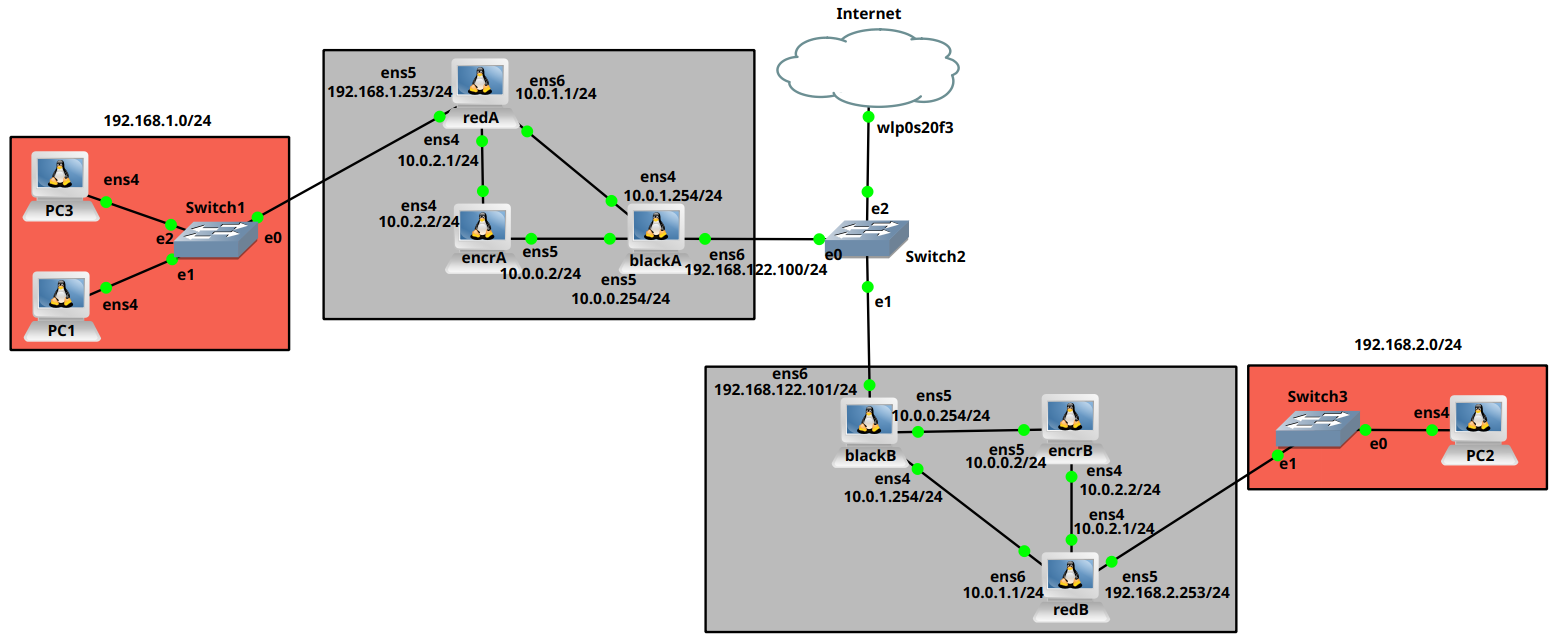
\includegraphics[width=0.95\textwidth]{images/gns3_2.png}
        \caption{Implementación de la propuesta de solución en GNS3.} 
    \end{figure}
    \end{column}
\end{columns}

    \note{Este proyecto surge como una posibilidad de abordar una solución de encriptación de redes de datos con un enfoque novedoso como es la segmentación virtual de dominios. 
    Además, es importante contar con una solución propia, cuyo desarrollo y mantenimiento no dependa de terceros y pueda ser auditada visto casos como el de Crypto AG, una empresa proveedora de equipos de cifrado con backdoors, que por mucho tiempo fue, en secreto, propiedad de entidades gubernamentales.}
\end{frame}

\begin{frame}{Pendientes}
    \begin{itemize}
        \item Validar el encriptador en ambiente virtualizado e implementarlo sobre hardware.
    \end{itemize}

    \note{Los objetivos del proyecto son desarrollar un sistema de comunicaciones seguras con segmentación virtual de dominios, implementar un encriptador de red seguro y confiable, probar la propuesta de solución en laboratorio virtual y documentar el proceso de desarrollo del proyecto.}
    
\end{frame}

\section{Revisión bibliográfica}

\begin{frame}{seL4}
    \begin{columns}
        \begin{column}{0.4\textwidth}
            \begin{itemize}
                \item Microkernel de código abierto.
                \item Formalmente probado.
                \item Hipervisor tipo 1.
                \item Aislamiento garantizado entre componentes.
            \end{itemize}
        \end{column}

        \begin{column}{0.6\textwidth}
            \begin{figure}
                \centering
                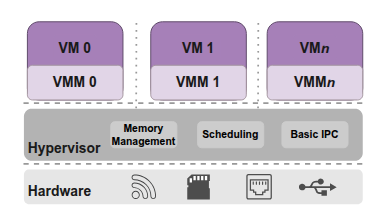
\includegraphics[width=\textwidth]{images/sel4scheme.png}
                \caption{Arquitectura de seL4 con VMM y máquinas virtuales.} 
            \end{figure}
        \end{column}
    \end{columns}
    
    \note{seL4 es un microkernel diseñado para ser seguro, eficiente y confiable. Se ejecuta directamente sobre hardware con capacidad de funcionar como hipervisor de tipo 1. Su característica más importante es la verificación formal de su funcionamiento, lo que significa que se demostró matemáticamente que su implementación cumple con sus especificaciones de diseño. Una de estas especificaciones críticas es la aislación entre componentes, fundamental para nuestro sistema de segmentación de dominios.}
\end{frame}

\begin{frame}{CAmkES}
    \begin{columns}
        \begin{column}{0.5\textwidth}
            \begin{itemize}
                \item \textbf{C}omponent \textbf{A}rchitecture for \textbf{m}icrokernel-based \textbf{E}mbedded \textbf{S}ystems.
                \item Framework de desarrollo para seL4.
                \item Arquitectura basada en componentes.
                \item Comunicación mediante interfaces bien definidas.
            \end{itemize}
        \end{column}

        \begin{column}{0.5\textwidth}
            \begin{figure}
                \centering
                % Aquí podrías agregar una imagen de la arquitectura CAmkES si la tienes
                \includegraphics[width=0.8\textwidth]{example-image}
                \caption{Arquitectura de componentes CAmkES.} 
            \end{figure}
        \end{column}
    \end{columns}
    
    \note{CAmkES es un framework que simplifica el desarrollo de sistemas sobre seL4. Permite diseñar aplicaciones como un conjunto de componentes que se comunican a través de interfaces bien definidas. Esto es especialmente útil para nuestro proyecto ya que cada máquina virtual puede ser vista como un componente independiente con interfaces de comunicación controladas, lo que facilita la implementación de la segmentación de dominios.}
\end{frame}

\begin{frame}{Modelo minimal\_64}
    \begin{columns}
        \begin{column}{0.5\textwidth}
            \begin{itemize}
                \item Ejemplo básico de CAmkES.
                \item Implementación mínima con máquinas virtuales de 64 bits.
                \item Punto de partida para el desarrollo.
                \item Configuración simple de red y sistema.
            \end{itemize}
        \end{column}

        \begin{column}{0.5\textwidth}
            \begin{figure}
                \centering
                \includegraphics[width=0.9\textwidth]{example-image}
                \caption{Arquitectura del modelo minimal\_64.} 
            \end{figure}
        \end{column}
    \end{columns}
    
    \note{El modelo minimal_64 es un ejemplo fundamental en CAmkES que proporciona una configuración básica para ejecutar máquinas virtuales de 64 bits sobre seL4. Este modelo incluye los componentes esenciales como el VMM (Virtual Machine Monitor) y una configuración mínima de red. Nos sirve como base para entender cómo estructurar nuestro sistema y como punto de partida antes de agregar la complejidad de la comunicación ZeroMQ y la funcionalidad de encriptación.}
\end{frame}

\begin{frame}{Modelo zmq\_samples}
    \begin{columns}
        \begin{column}{0.5\textwidth}
            \begin{itemize}
                \item Ejemplo de implementación en CAmkES.
                \item Comunicación entre máquinas virtuales usando ZeroMQ.
                \item Patrón de mensajería asíncrona.
                \item Base para la implementación del encriptador.
            \end{itemize}
        \end{column}

        \begin{column}{0.5\textwidth}
            \begin{figure}
                \centering
                % Aquí podrías agregar un diagrama del modelo zmq_samples
                \includegraphics[width=0.9\textwidth]{example-image}
                \caption{Modelo de comunicación zmq\_samples.} 
            \end{figure}
        \end{column}
    \end{columns}
    
    \note{El modelo zmq_samples es un ejemplo práctico que demuestra cómo implementar comunicación segura entre máquinas virtuales en seL4 usando ZeroMQ. Este modelo nos sirve como punto de partida para implementar la comunicación entre los dominios rojo y negro de nuestro encriptador, manteniendo el aislamiento necesario mientras permite el intercambio controlado de información.}
\end{frame}



\section{Desarrollo}

\begin{frame}{Estrategia de modelos en entornos virtualizados}
   \begin{itemize}
       \item \textbf{¿Qué?}: Realizar modelos que validen progresivamente los componentes desarrollados.
       \item \textbf{¿Para qué?}: 
       \begin{itemize}
        \item Ligar problemas concretos a cada modelo y resolverlos de forma independiente.
        \item Implementar un encriptador funcional en un entorno virtualizado como paso previo a su despliegue en hardware.
       \end{itemize}
       
   \end{itemize}
\end{frame}

\begin{frame}{Modelo I: Arquitectura lógica}
    \begin{columns}
        \begin{column}{0.4\textwidth}
            \begin{itemize}
                \item Validar la arquitectura lógica de tres VMs.
                \item 
            \end{itemize}
        \end{column}
        \begin{column}{0.6\textwidth}
            \begin{figure}
                \centering
                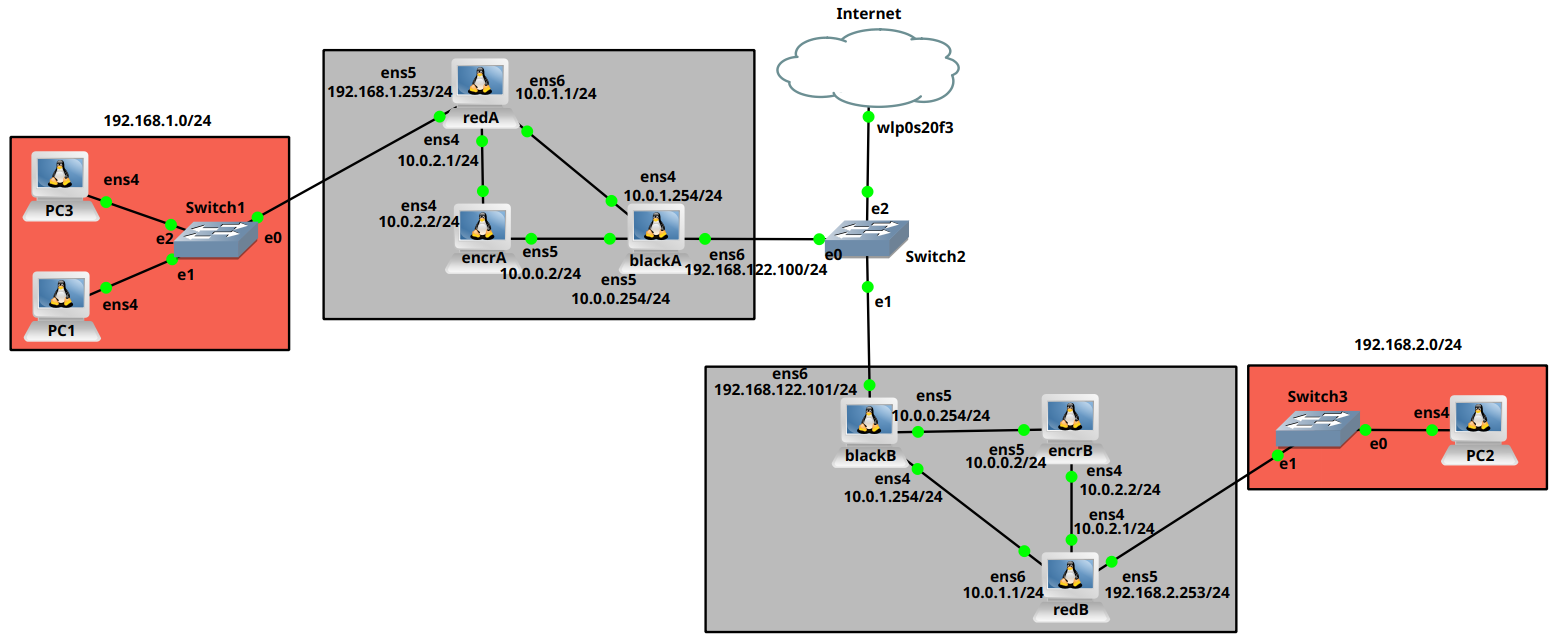
\includegraphics[width=\textwidth]{images/gns3_2.png}
                \caption{Arquitectura lógica en GNS3.}
            \end{figure}
        \end{column}
    \end{columns}
\end{frame}

\begin{frame}{Modelo II: seL4 como hipervisor}
    \begin{columns}
        \begin{column}{0.4\textwidth}
            \begin{itemize}
                \item
            \end{itemize}
        \end{column}
        \begin{column}{0.6\textwidth}
            \begin{figure}
                \centering
                \includegraphics[width=0.5\textwidth]{example-image}
                \caption{Algo}
            \end{figure}
        \end{column}
    \end{columns}
\end{frame}

\begin{frame}{Modelo II: seL4 como hipervisor - Sistema operativo VMs}
    
\end{frame}

\begin{frame}{Modelo II: seL4 como hipervisor - Gestión de memoria VMs}
    
\end{frame}

\begin{frame}{Modelo II: seL4 como hipervisor - Passthrough de hardware}
    
\end{frame}

\begin{frame}{Modelo III: Encriptador en seL4}
    \begin{columns}
        \begin{column}{0.4\textwidth}
            \begin{itemize}
                \item
            \end{itemize}
        \end{column}
        \begin{column}{0.6\textwidth}
            \begin{figure}
                \centering
                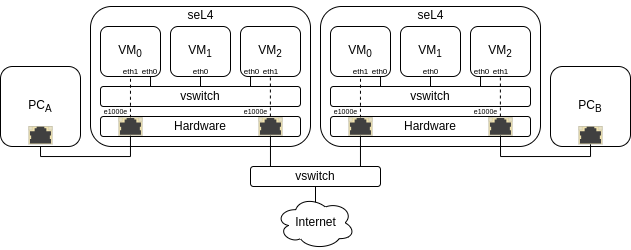
\includegraphics[width=\textwidth]{images/3_model4.png}
                \caption{Algo.}
            \end{figure}
        \end{column}
    \end{columns}
\end{frame}

\begin{frame}{Modelo III: Encriptador en seL4 - Comunicación entre VMs}

\end{frame}

\begin{frame}{Modelo III: Encriptador en seL4 - Integración}
% Mostrar ping entre PCs
\end{frame}

\begin{frame}{Implementación en hardware}
    \begin{columns}
        \begin{column}{0.4\textwidth}
            \textbf{Desafíos:}
            \begin{itemize}
                \item[\space \textcolor{green}{\checkmark}] Redirección de consola.
                \item[{\color{red}\texttimes}] Passthrough de controlador Ethernet.
                \item[{\color{red}\texttimes}] Throughput entre VMs.
            \end{itemize}
        \end{column}

        \begin{column}{0.5\textwidth}
            \begin{figure}
                \centering
                \includegraphics[width=0.8\textwidth]{example-image}
                \caption{SuperMicro SYS-E300-9D.} 
            \end{figure}
        \end{column}
    \end{columns}

\end{frame}


\section{Conclusiones}
\begin{frame}{Conclusiones}
    \begin{itemize}
        \item Avance significativo en la implementación de un sistema de comunicaciones seguras.
        \item Validación de la arquitectura lógica y funcionalidad de los modelos.
        \item Próximos pasos: implementación en hardware y pruebas de integración.
    \end{itemize}

    \note{En resumen, hemos avanzado significativamente en el desarrollo de un sistema de comunicaciones seguras con segmentación virtual de dominios. Hemos validado la arquitectura lógica y la funcionalidad de los modelos, lo que nos permite avanzar hacia la implementación en hardware y las pruebas de integración.}
\end{frame}

\begin{frame}
    \begin{center}
        \Huge ¡Muchas gracias! \\
        \Huge ¿Preguntas?
    \end{center}
\end{frame}

% FIN

\end{document}